% !TeX root = ../main.tex
% !TEX root = ../main.tex
% -*- root: ../main.tex -*-
% -*- program: pdflatex -*-
\chapter{利用样条插值方法对~MRPC~进行刻度}

在上一章中讲到,~MRPC-TOF~直接测量的信息包括原始的飞行时间和过阈时间(~time-over-threshold~,简称~TOT~)。为了得到精确的飞行时间信息,还需要对粒子在读数条上的传播时间,过阈时间前沿的晃动以及在电缆的时间延迟等因素进行刻度和修正,需要进行离线分析。为了得到良好的时间分辨,需要利用刻度样本进行离线刻度和修正,得到相应的刻度常数,再对原始数据进行重建,进而得到飞行时间探测器的性能。

~MRPC-TOF~的离线刻度是通过比较测量时间~$t_{mea}=t_{raw}-t_{0}-t_{cor}$~与带电粒子从对撞顶点到击中~MRPC-TOF~的预期飞行时间~$t_{exp}=L/\beta c$~来比较,其中~$t_{raw}$~是飞行时间探测器电子学测得的原始的时间;$t_{0}$~是事例的起始时间,可以由事例起始时间算法给出;$t_{cor}$~是时间的修正项;c~是真空中的光
速;$\beta=p/\sqrt{p^2+m^2}$是带电粒子的飞行速度;m~是粒子的质量;飞行长度~L~和动量~P~是通过主漂移室(~MDC~)测量得到的。

时间修正项~$t_{cor}$~是过阈时间(TOT)和击中位置(z)的函数。对于击中位置项,信号击中读数条的位置不同,则在读数条上的传播时间不同,在上一章的讨论中知道,时间随击中位置的变化近似线性,它们之间的斜率对应读数条中信号传播的有效速度。对于过阈时间,由于过阈和反射问题的存在,时间对过阈时间的分布呈现折线型,这种分布难以采用有效的函数进行拟合。这是刻度研究中的重点和难点部分。

\begin{comment}
对于每一个读数条,每个读出单元定义:
%\begin{equation}
\begin{displaymath}
\chi^2(counter,readout)=\sum\limits_{event}(t_{mea}-t_{exp})^2
\end{displaymath}
%\end{equation}
通过分析大量的事例样本,进行反复迭代,利用最小~$\chi^2$~方法,刻度常数项可以通过~$\partial\chi^2/\partial P_{i}=0$~得到。在重建中,利用刻度得到的刻度常数对原始的飞行时间信息进行重建,就可以得到经过刻度修正得到的飞行时间信息。
\end{comment}

STAR~实验~MRPC~采用的是样条插值(~spline Fit~)刻度的方法。在第一章关于论文的国内外研究进展中介绍了~STAR~实验的过阈时间也存在多峰现象,也是因为反射现象造成的,这一点和我们~BESIII~实验的~MRPC-TOF~的过阈时间的多峰问题类似,因此本文也首先对~BESIII~的~MRPC~进行了样条插值方法的研究。

本章主要介绍样条插值方法。分两部分介绍:先对过阈时间进行插值,之后对击中位置修正(对应STAR实验的刻度方法);先对击中位置进行修正,之后对过阈时间进行插值。并进行了一定的结果比较,发现先修正击中位置,然后对过阈时间进行插值的结果比另一种方法好。

样条插值方法优点:光滑性好,且低阶就能拟合的很好。高能所集群下的~root~中有关于~TSpline~的类包,可以利用它完成样条插值的拟合。

本章数据选用的是~2016~年~5~月~24~日到~5~月~30~日这期间~BESIII~对撞数据中的~Bhabha~事例。选用~Bhabha~事例是因为它事例量大,易于挑选,纯度高,适合做刻度样本。

%%%%%%%%%%%%%%%%%%%%%%%%%%%%%%%%%%%%%%%%%%%%%%%%%%%%%%%%%%%%%%%%%%%%%%%%%%%%%%
\section{修正击中位置前进行插值}
%%%%%%%%%%%%%%%%%%%%%%%%%%%%%%%%%%%%%%%%%%%%%%%%%%%%%%%%%%%%%%%%%%%%%%%%%%%%%%

本节以挑选的~Bhabha~事例中击中MRPC-TOF读数条位置在~MRPC~中模块编号为~55~,对数条编号为~7~这一个读数条为例。首先按照~STAR~实验的做法进行刻度研究。具体做法,就是先对过阈时间进行插值修正,之后对得到的结果再次进行击中位置修正得到最终的时间分辨等刻度信息。
\subsection{等事例数分~bin~拟合}
\begin{itemize}
    \item 以过阈时间的大小为量对所选的事例数进行等事例数分~bin~
    \item 对于每个~bin~区间,进行拟合
    \item 对于上一步得到的中心值进行插值,得到插值的刻度常数
    \item 利用上一步得到的刻度常数,对时间信息进行修正 
\end{itemize}

等事例数分~bin~的原因是时间随过阈时间的分布是不均匀的。在过阈时间很小或者很大的部分事例数很少,如果采用等区间分~bin~的话,会出现比较大的误差棒。

\begin{figure}[htbp]
\begin{minipage}[t]{0.5\linewidth}
%\centering
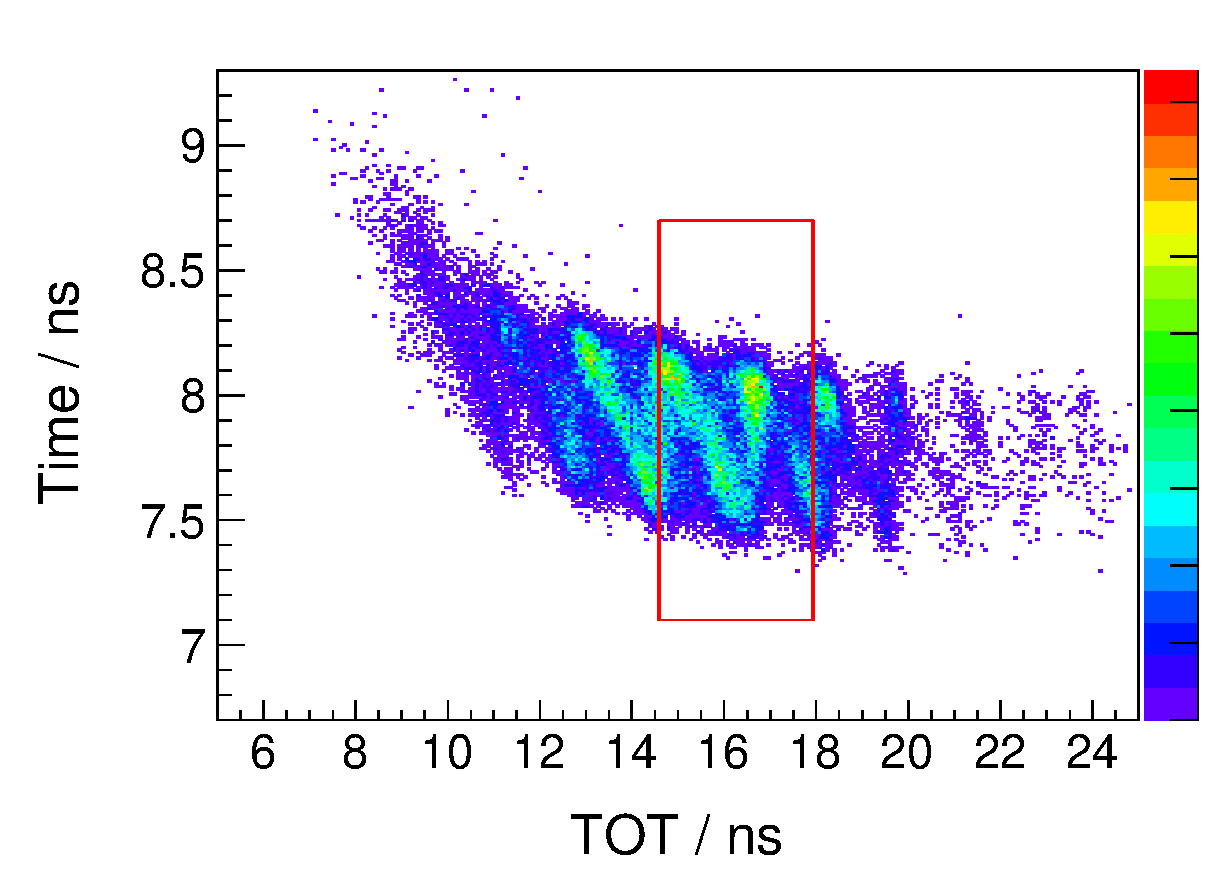
\includegraphics[width=0.9\textwidth]{chap2/ScatterDiagram.eps}
\subcaption{时间对TOT的分布}
\label{fig:ScatterDiagram}
\end{minipage}%
\hfill
\begin{minipage}[t]{0.5\linewidth}
%\centering
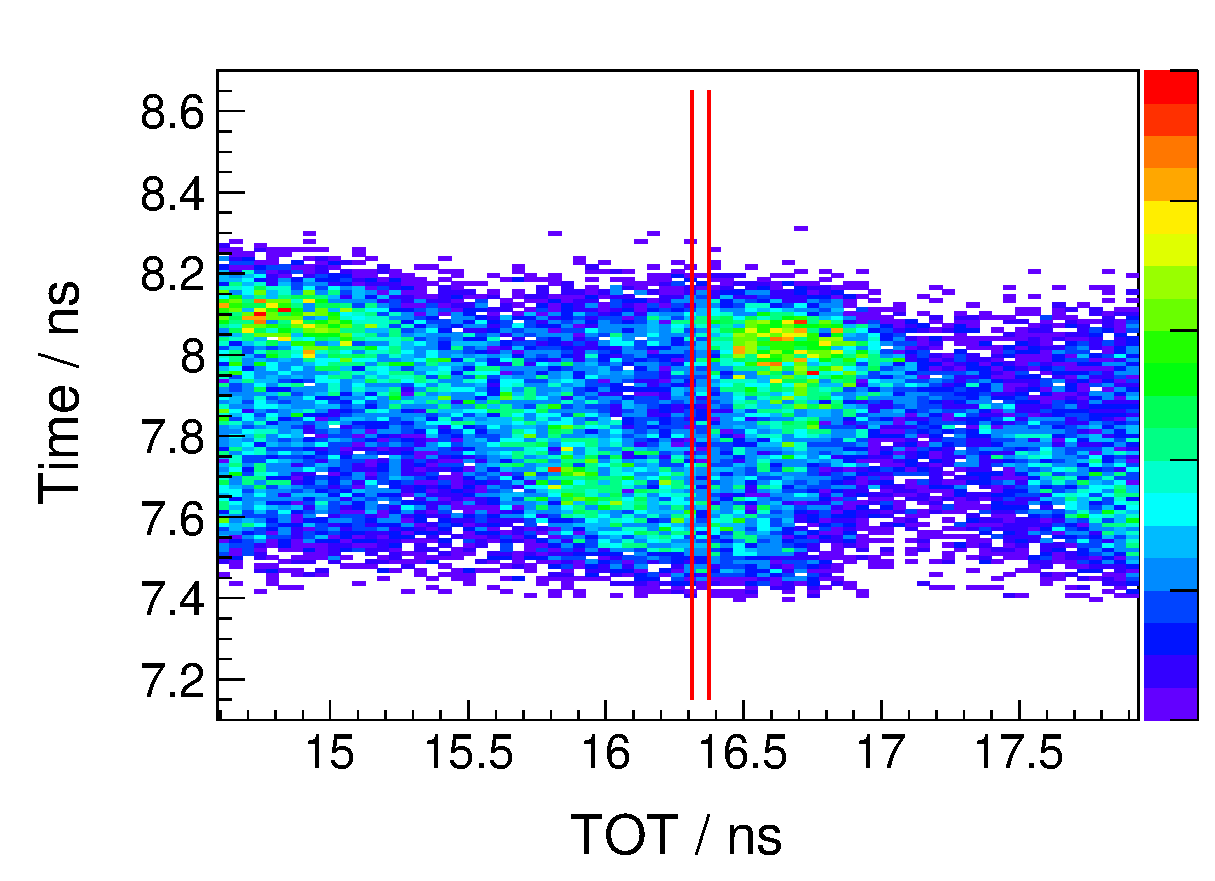
\includegraphics[width=0.9\textwidth]{chap2/cutScatterDiagram.eps}
\subcaption{截取时间对过阈时间的分布}
\label{fig:cutScatterDiagram}
\end{minipage}
\caption{时间对过阈时间的分布}
%\label{fig:Diagram}
\end{figure}
\begin{figure}[htbp]
\centering
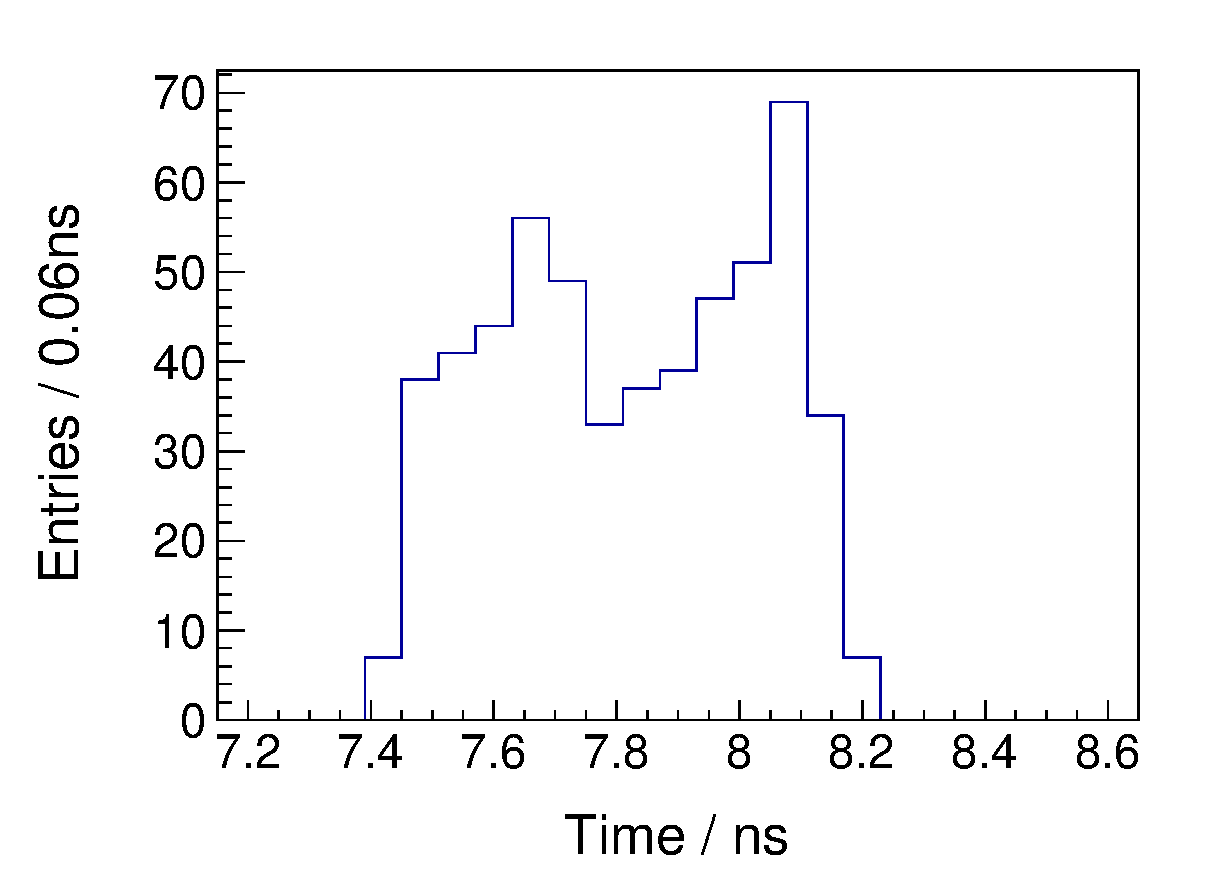
\includegraphics[width=0.45\textwidth]{chap2/onebinTime.eps}
\caption{截取一个bin的时间分布(对应两个峰值)}
\label{fig:onebinTime}
\end{figure}


分~bin~完成后,发现一个~bin~内时间有两个峰值(如图~\ref{fig:onebinTime}~)。图~\ref{fig:ScatterDiagram}~是时间对过阈时间的分布,图~\ref{fig:cutScatterDiagram}~是图~\ref{fig:ScatterDiagram}~截取的一部分的分布。
图~\ref{fig:onebinTime}~是一个bin内的时间分布,可以明显看出具有双峰。对此,找不到合适的函数可以在一个区间内得到一个合适的中心值。

\subsection{两个高斯拟合和单个高斯拟合}

在上一节中时间与过阈时间的的散点图中,已经看到分~bin~后一个~bin~区间中对应两个时间峰值。因此首先考虑对每个区间采取两个高斯函数进行拟合,并得到对应的两个中心值。然后选取两个高斯占比例高的($>$50$\%$)对应的中心值作为插值拟合的插值点进行插值,发现最终得到的时间分辨效果很差。之后考虑对每个区间直接采用高斯拟合得到中心值(这个中心值在采用两个高斯拟合得到的两个中心值之间)进行插值拟合。并与上一个方法进行对比。具体做法如下:

图~\ref{fig:double-ScatterDiagram}~,~\ref{fig:single-ScatterDiagram}~分别是对每个~bin~用两个高斯和一个高斯函数拟合后得到的中心值的分布

\begin{figure}[!h]
\begin{minipage}[!h]{0.5\linewidth}
%\centering
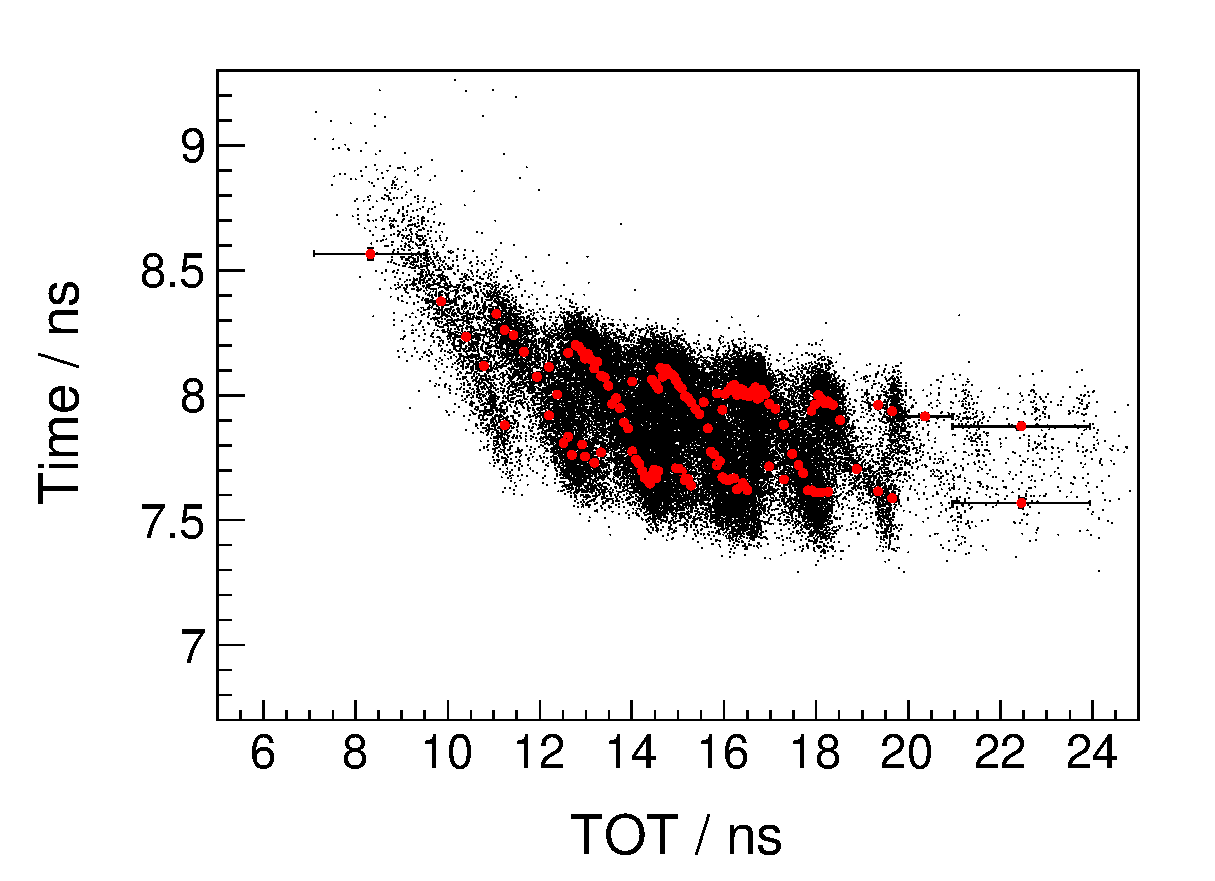
\includegraphics[width=0.9\textwidth]{chap2/double-ScatterDiagram.eps}
\subcaption{两个高斯拟合后的graph图}
\label{fig:double-ScatterDiagram}
\end{minipage}%
\hfill
\begin{minipage}[!h]{0.5\linewidth}
%\centering
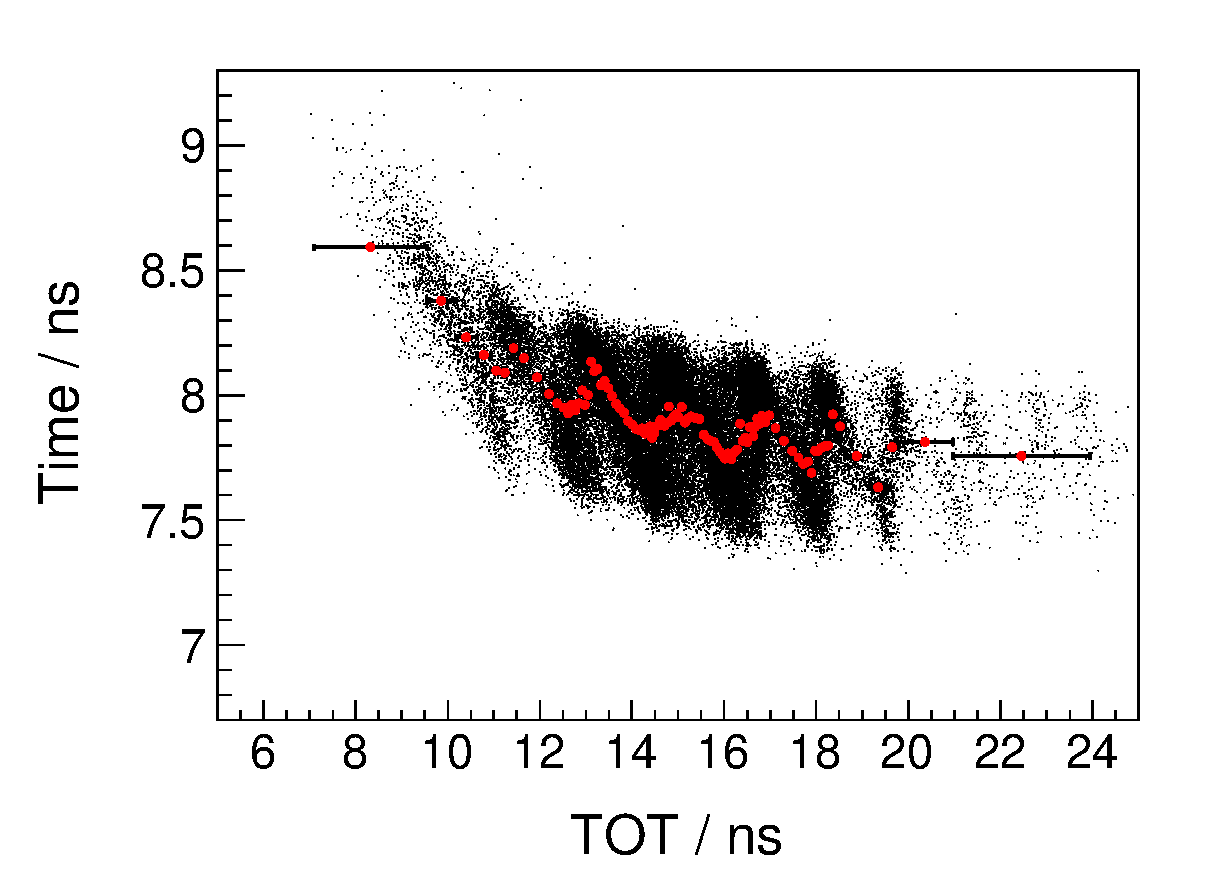
\includegraphics[width=0.9\textwidth]{chap2/single-ScatterDiagram.eps}
\subcaption{一个高斯拟合后的graph图}
\label{fig:single-ScatterDiagram}
\end{minipage}
\caption{高斯拟合后的graph}
\end{figure}


%对比看出,右图的拟合更符合原来散点的分布情况。

\begin{figure}[!h]
\begin{minipage}[!h]{0.5\linewidth}
%\centering
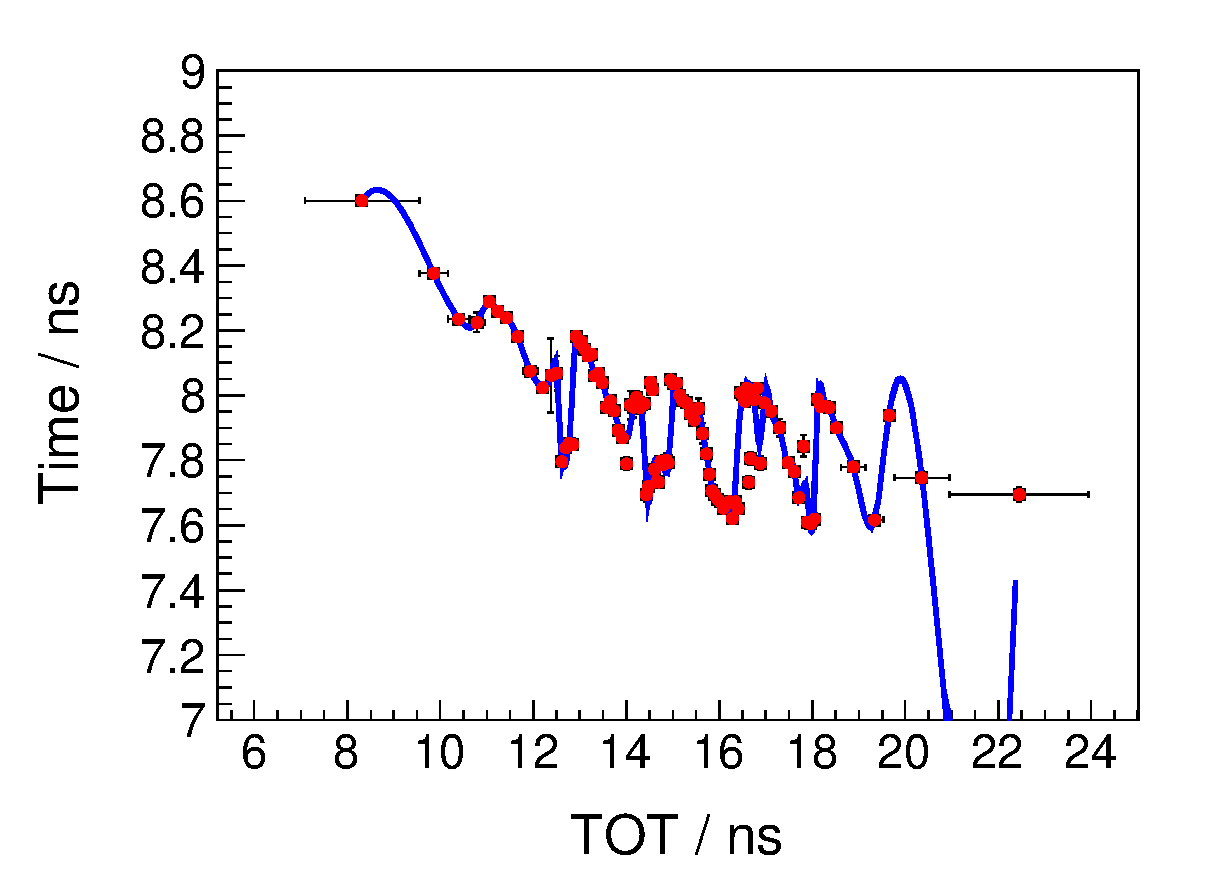
\includegraphics[width=0.9\textwidth]{chap2/double-leftspline.eps}
\subcaption{两个高斯拟合得到的中心值的样条插值}
\label{fig:double-leftspline}
\end{minipage}%
\hfill
\begin{minipage}[!h]{0.5\linewidth}
%\centering
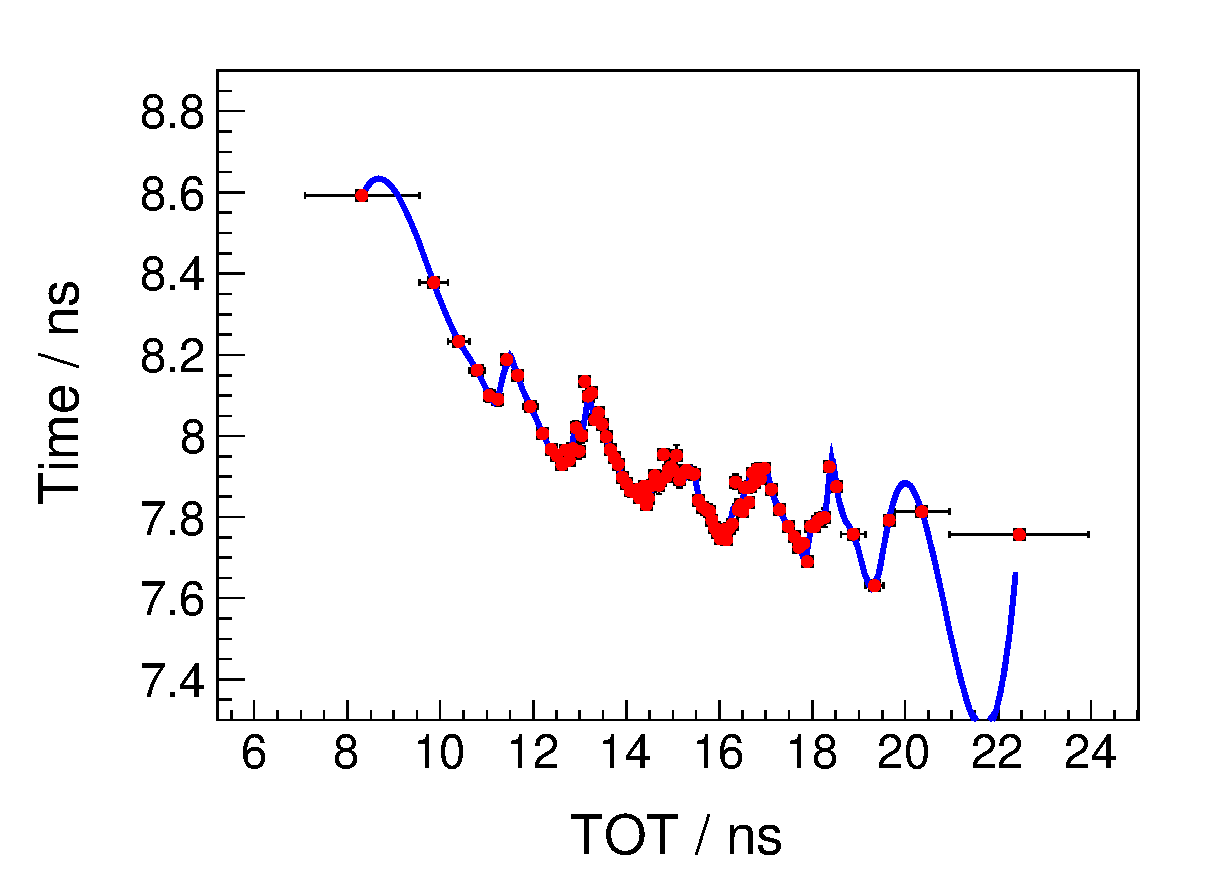
\includegraphics[width=0.9\textwidth]{chap2/single-leftspline.eps}
\subcaption{一个高斯拟合得到的中心值的样条插值}
\label{fig:single-leftspline}
\end{minipage}
\caption{样条插值}
\end{figure}
图~\ref{fig:double-leftspline}~第一种做法的样条插值曲线,对于每个~bin~的时间的中心值取相对比例高的那一个。图~\ref{fig:single-leftspline}~第二种做法的样条插值曲线。

\subsection{击中位置的修正}
上述两种方法,插值修正完过阈时间后,时间随击中位置的分布还有依赖(如图~\ref{fig:after-spline-fit-TOT-tVSz}~),对此进行一个多项式修正,然后得到最终时间分辨。

\begin{figure}[!h]
  \centering
  \includegraphics[width=0.9\textwidth]{chap2/after-spline-fit-TOT-tVSz.eps}
  \caption{对过阈时间采用样条插值修正后时间对击中位置的分布}
  \label{fig:after-spline-fit-TOT-tVSz}
\end{figure}
%图~\ref{fig:after-spline-fit-TOT-tVSz}~中,时间与击中位置之间的关系近似线性,采用多项式拟合。

\begin{figure}[!h]
\begin{minipage}[!h]{0.48\linewidth}
\centering
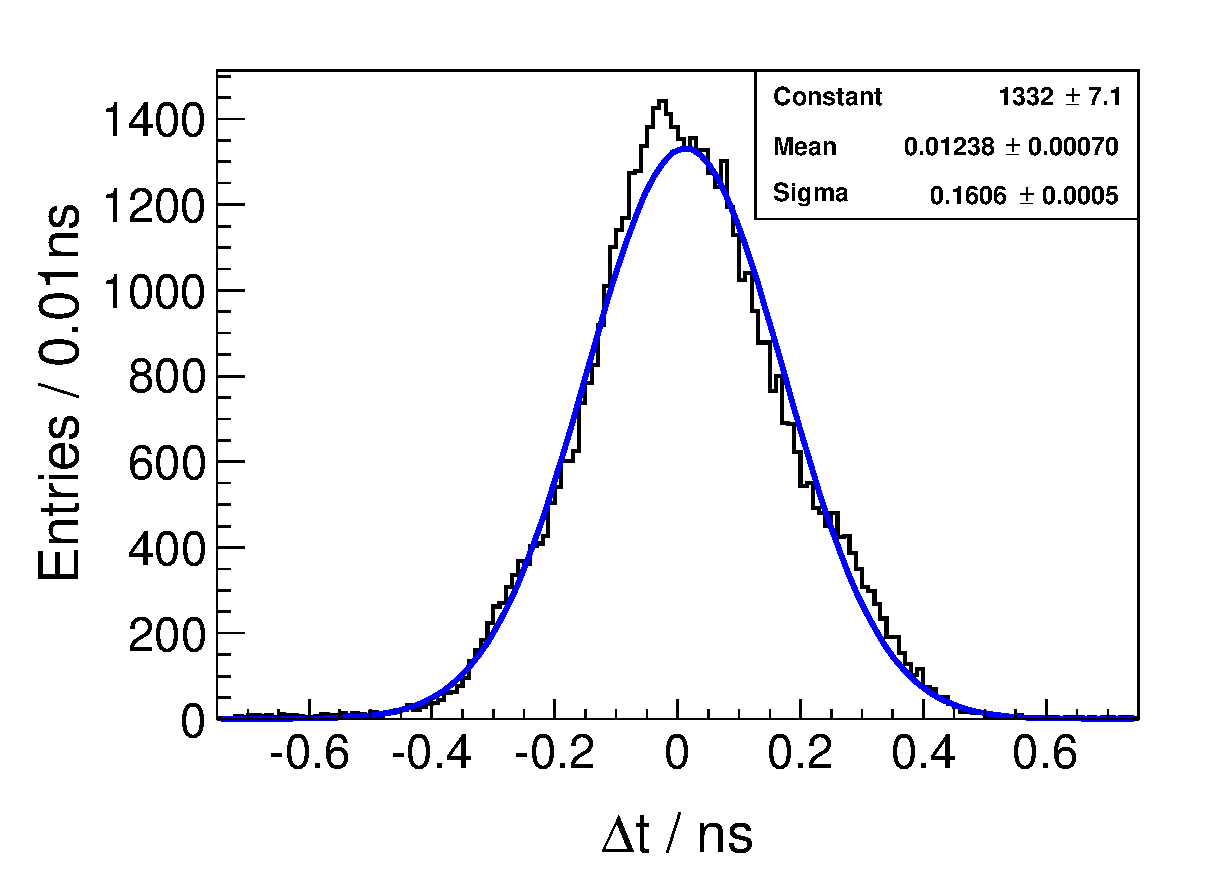
\includegraphics[width=0.9\textwidth]{chap2/double-resolutiongauss.eps}
\subcaption{时间分辨1}
\label{fig:double-resolutiongauss}
\end{minipage}%
\hfill
\begin{minipage}[!h]{0.48\linewidth}
\centering
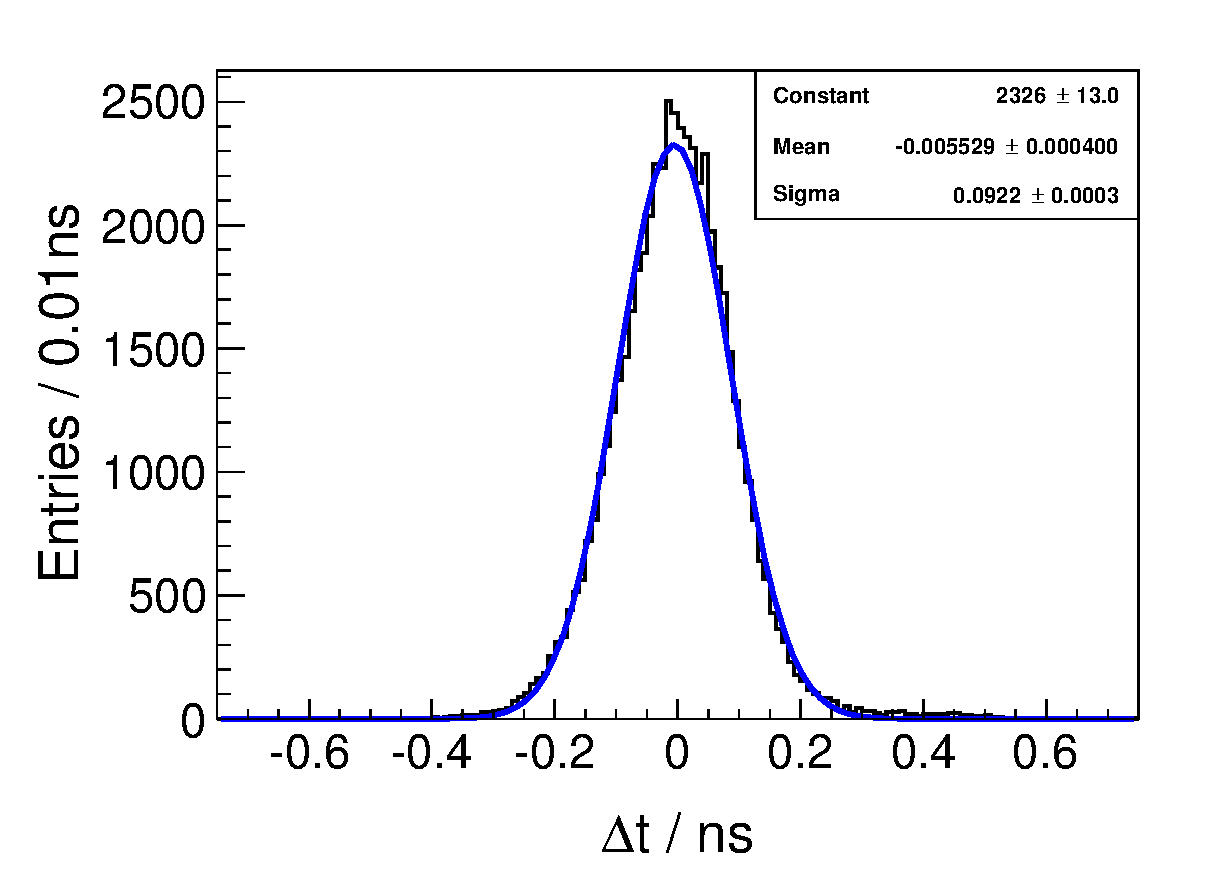
\includegraphics[width=0.9\textwidth]{chap2/single-resolutiongauss.eps}
\subcaption{时间分辨2}
\label{fig:single-resolutiongauss}
\end{minipage}
\caption{时间分辨}
\end{figure}

图~\ref{fig:double-resolutiongauss}~是第一种做法得到的时间分辨,为~160~ps;图~\ref{fig:single-resolutiongauss}~是第二种做法得到的时间分辨,为~92~ps。这个结果和下一节先修正击中位置后修正过阈时间的结果相比,差别很大。

分析原因:在上一章中介绍反射问题时讲到,过阈时间(TOT)的多峰来自反射。一次反射内,时间对过阈时间的依赖近似线性关系,样条插值的光滑性决定不能完全描述这种关系。

\begin{comment}

\subsection{反射问题}
图~\ref{fig:TOT}~是信号的过阈时间。对于一定的阈值,幅度大小不同的信号,对应的过阈时间不同。信号幅度越大,过阈时间也就越大。
图~\ref{fig:reflection}~是~MRPC~读数条的反射问题,分为近端反射和远端反射。由于读数条本身较短,反射信号只是比真实信号时间晚不到1ns,这样导致反射信号和原来的真实信号叠加。测量的过阈时间也就变大了。
正是由于过阈问题和反射问题的存在,导致时间对过阈时间的分布复杂。对时间和过阈时间的关系的研究也刻度研究的重点和难点部分。

\begin{figure}[!h]
\begin{minipage}[!h]{0.5\linewidth}
%\centering
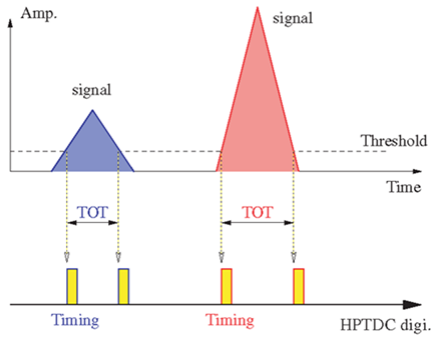
\includegraphics[width=0.8\textwidth]{chap2/TOT.png}
\subcaption{过阈时间~\cite{Shao:2009aa}~}
\label{fig:TOT}
\end{minipage}
\hfill
\begin{minipage}[!h]{0.5\linewidth}
%\centering
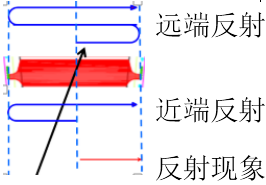
\includegraphics[width=0.9\textwidth]{chap2/reflection.png}
\subcaption{反射问题}
\label{fig:reflection}
\end{minipage}%
\caption{反射问题和过阈时间}
\end{figure}

\end{comment}
%%%%%%%%%%%%%%%%%%%%%%%%%%%%%%%%%%%%%%%%%%%%%%%%%%%%%%%%%%%%%%%%%%%%%%%%%%%%%%%
\section{修正击中位置后进行插值}
%%%%%%%%%%%%%%%%%%%%%%%%%%%%%%%%%%%%%%%%%%%%%%%%%%%%%%%%%%%%%%%%%%%%%%%%%%%%%%
上一小节采用的是~STAR~实验关于~MRPC-TOF~离线数据刻度方法,效果并不好。在论文第二章中关于反射部分的分析指出,在~BESIII~实验中的~MRPC-TOF~的过阈时间和击中位置之间存在依赖。这种依赖正是来自信号在读数条中的反射。基于此,采用先对击中位置进行修正,然后对过阈时间进行修正的方法。
\subsection{击中位置的修正后,时间对过阈时间的分布}
图~\ref{fig:t2q}~给出了修正击中位置前后,时间对过阈时间的分布变化。其中图~\ref{fig:q-before}~表示修正击中位置前,图~\ref{fig:q-after}~表示修正击中位置后。容易看出,修正完击中位置后时间对过阈时间的折线几乎消失。在此基础上,对过阈时间进行插值拟合。
\begin{figure}[!h]
\begin{minipage}[!h]{0.5\linewidth}
%\centering
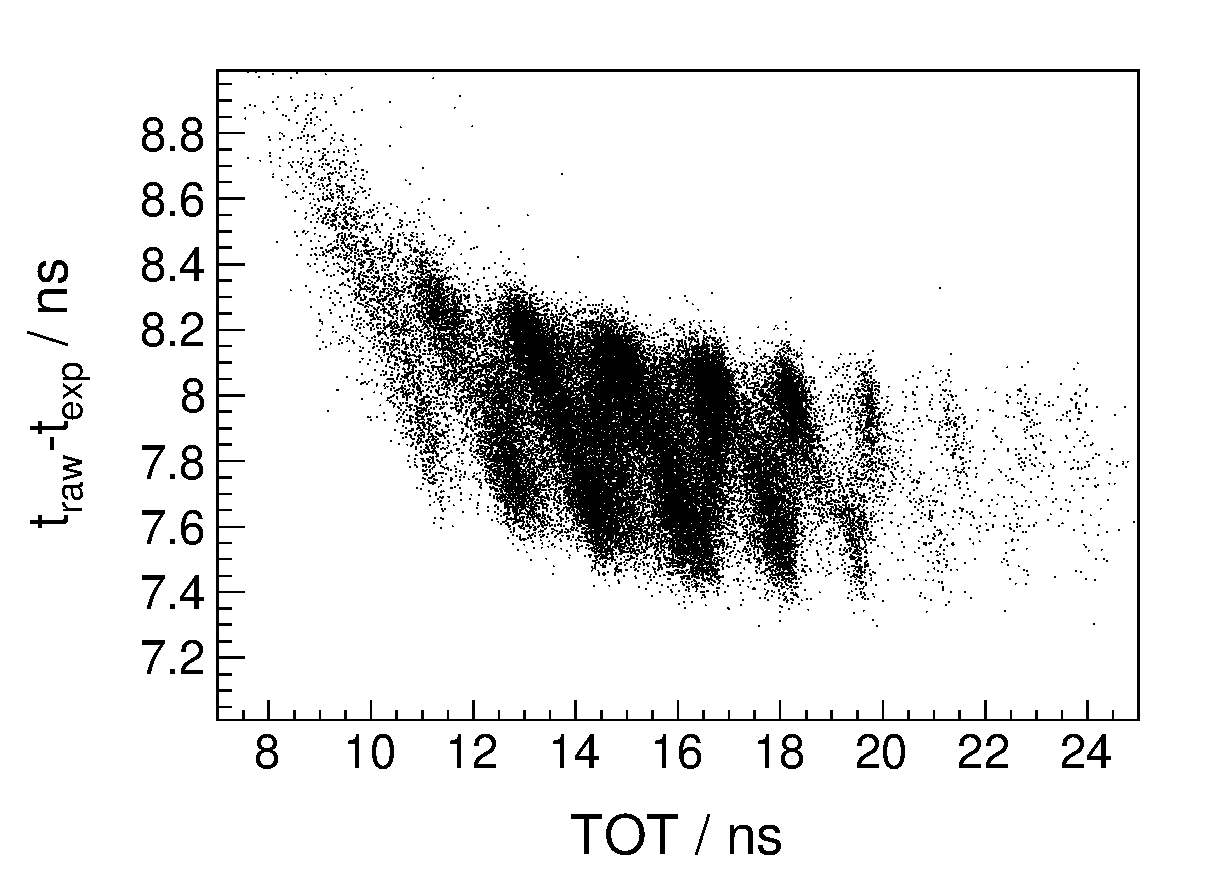
\includegraphics[width=0.9\textwidth]{chap2/q-before.eps}
\subcaption{击中位置修正前}
\label{fig:q-before}
\end{minipage}%
\hfill
\begin{minipage}[!h]{0.5\linewidth}
%\centering
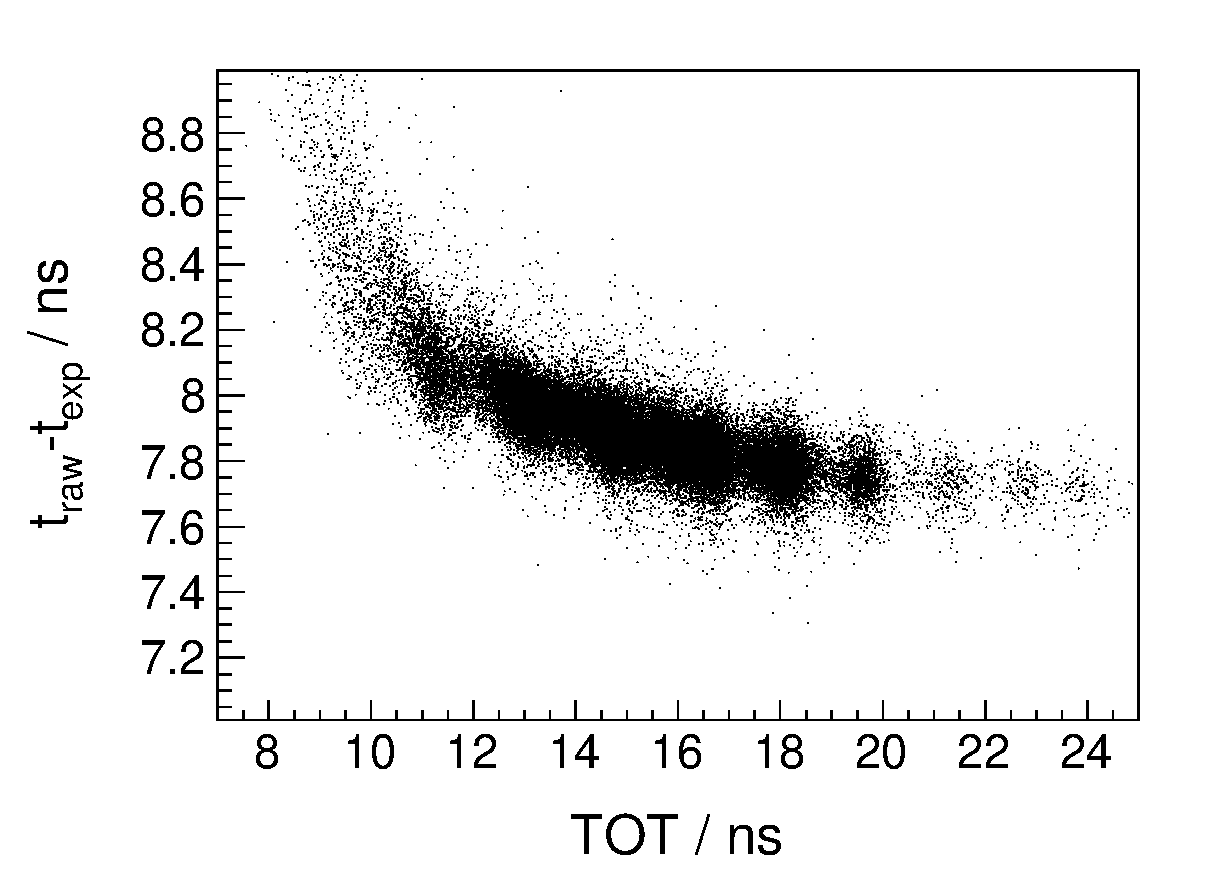
\includegraphics[width=0.9\textwidth]{chap2/q-after.eps}
\subcaption{击中位置修正后}
\label{fig:q-after}
\end{minipage}
\caption{击中位置修正前后时间对过阈时间的分布}
\label{fig:t2q}
\end{figure}

\subsection{修正击中位置后对过阈时间插值}

\begin{figure}[!h]
\begin{minipage}[!h]{0.5\linewidth}
%\centering
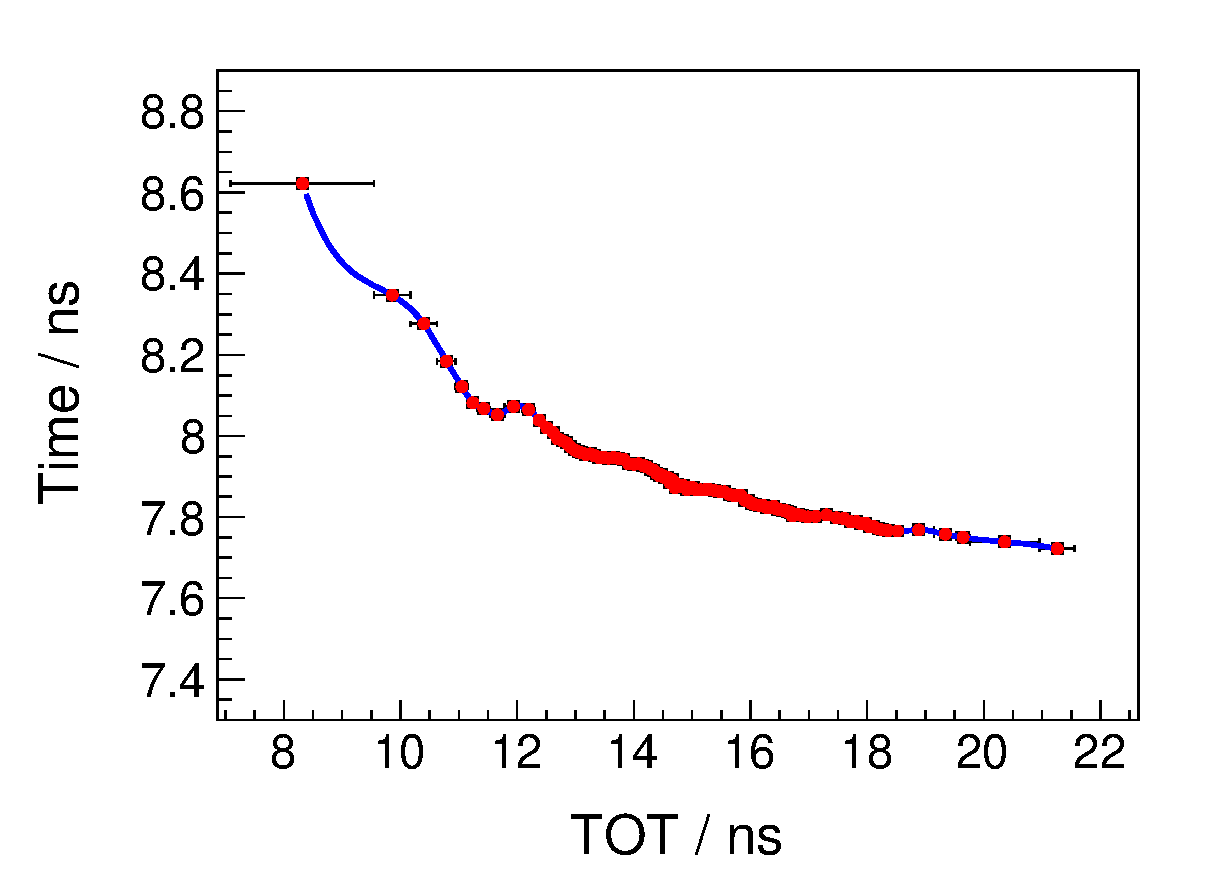
\includegraphics[width=0.9\textwidth]{chap2/after-left-spline.eps}
\subcaption{击中位置修正后对过阈时间进行插值}
\label{fig:after-left-spline}
\end{minipage}%
\hfill
\begin{minipage}[!h]{0.5\linewidth}
%\centering
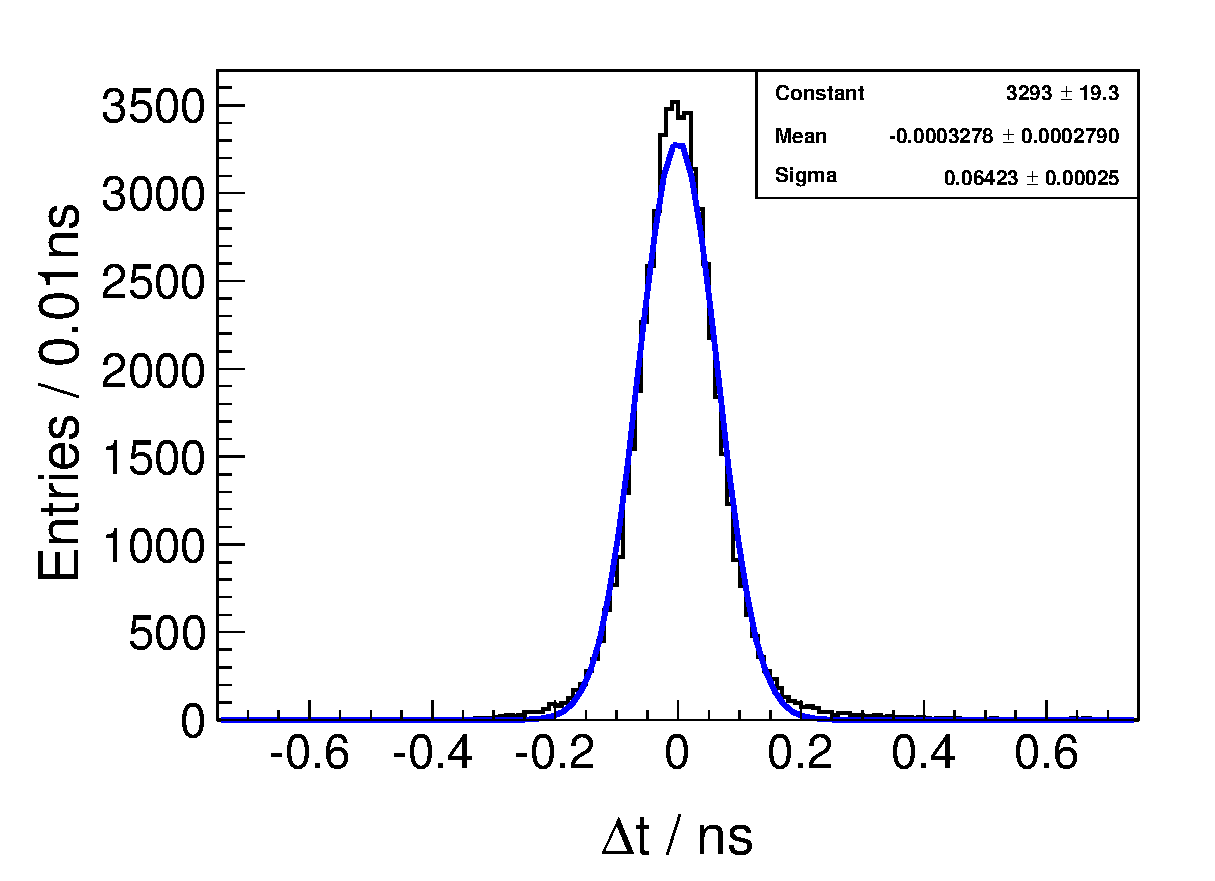
\includegraphics[width=0.9\textwidth]{chap2/resolutiongauss.eps}
\subcaption{时间分辨}
\label{fig:resolutiongauss}
\end{minipage}
\caption{击中位置修正后插值}
\end{figure}

对~\ref{fig:t2q}~进行插值拟合,如图~\ref{fig:after-left-spline}~;图~\ref{fig:resolutiongauss}~是这种方法得到的最终的时间分辨,为~64~ps,比之前先对过阈时间进行插值修正然后对击中位置进行修正得到的时间分辨(160~ps,92~ps)好。

出现这种结果的原因是在于先修正击中位置的贡献后,时间对过阈时间的依赖关系变得简单,在此基础上进行插值拟合效果变好。
这种对比也说明了先对击中位置进行修正,之后再对过阈时间进行修正是应该采取的修正顺序。

\section{小结}

~STAR~实验中关于~MRPC-TOF~中的过阈时间的多峰问题的产生机制和我们~BESIII~实验的~MRPC-TOF~的过阈时间的多峰问题类似。STAR~实验对此刻度采用的是样条插值方法,先对过阈时间进行修正,然后对击中位置进行修正。

本章利用样条插值方法,首先介绍~STAR~实验在~BESIII~实验的~MRPC-TOF~离线数据刻度中的实际效果,发现在处理过阈时间问题上效果不好,得到的时间分辨不好。分析原因是来自于信号在读数条中的反射。这种反射导致时间对过阈时间的分布出现折线状,折线部分是线性的。样条插值的光滑性导致不能完全描述这种情况。基于此,采用先对击中位置进行修正的方法,发现修正后时间对过阈时间的分布的折线状况几乎消失,然后对过阈时间进行插值拟合。并对这两种方法得到的时间分辨进行比较。得出应该先进行击中位置的修正,然后进行过阈时间的插值拟合修正。
